
% non contare la pagina del titolo
\pagenumbering{gobble}

% titolo
\thispagestyle{empty}

\vspace*{-2.5cm} 
\mdseries{

\begin{center}
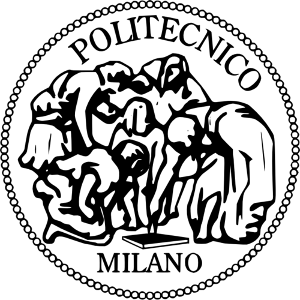
\includegraphics[width=5cm]{logo.png}

\vspace*{0.6cm}
{\Large\textsc{Politecnico di Milano}}\\
\rule{7cm}{1pt}

\vspace*{0.5cm}

Corso di Laurea Triennale in \textsc{Ingegneria Matematica}\\
Scuola di \textsc{Ingegneria Industriale e dell'Informazione}\\
\vspace*{1.3cm} 
{\LARGE\textmd{\textbf{
Sull'esistenza di soluzioni locali\\di equazioni differenziali\\\vspace*{0.2cm} alle derivate parziali
}}}

\vspace*{1.5truecm} 

{\small Tesi di}
{\large\vspace*{0.3cm}\\Alessandro Pedone}

\vspace*{1.3cm}

\begin{tabular}{@{}ll}
\small
Relatore:\\[0.5cm]
\normalsize
\quad Prof. Maurizio Grasselli & .......................................\\[1cm]
\small
Candidato:\\[0.5cm]
\normalsize
\quad Alessandro Pedone & .......................................\\
\end{tabular}
\vfill
\rule{6cm}{1pt}

\small
Sessione di Laurea Settembre 2024\\
Anno Accademico 2023/2024
\end{center} 
\clearpage
}
\blankpage

% conta con i numeri romani 
\pagenumbering{roman}

% citazione
\setlength\epigraphwidth{8cm}
\setlength\epigraphrule{0pt}
\vspace*{\fill}
\epigraph{\textit{All his life -- he had difficulty saying this, as he admitted, being always wary of too much enthusiasm -- all his life he had been waiting for such a student to come into this room. A student who would challenge him completely, who was not only capable of following the strivings of his own mind but perhaps of flying beyond them.}}{--- \textup{Alice Munro}, \textit{Too Much Happiness}}
\vspace*{\fill}
%indice
\tableofcontents

\newpage
\blankpage